\documentclass{article}
\usepackage[utf8x]{inputenc} % codifica scrittura
\usepackage[nochapters]{classicthesis} % nochapters

\usepackage[T1]{fontenc}
\usepackage[square,numbers]{natbib}
\usepackage{amsmath, amsthm, amssymb, amsfonts, tikz}
\usetikzlibrary{snakes}
\usepackage{titletoc}
\usepackage{verbatim}
\usepackage{hyperref}
\usepackage{boxedminipage}

\titlecontents{section}[3em]{}{\contentslabel{1em}}{}{\titlerule*[1.5pc]{.}\contentspage}
\titlecontents{subsection}[6em]{}{\contentslabel{2em}}{}{\titlerule*[1.5pc]{.}\contentspage}

\begin{document}

\title{\rmfamily\normalfont\spacedallcaps{Computer Aided Graphic
    Design course exercises}}

\author{\spacedlowsmallcaps{Massimo Nocentini}}
\date{\today}

\maketitle


\begin{abstract}
  This document contains some exercises and collects my work done during
  the CAGD course given by Prof. Alessandra Sestini and Prof. Costanza
  Conti at University of Florence.

  In particular, this document collect exercises requested by Prof.
  Costanza Conti about Bezier and BSplines curves. We implement numerical
  methods using Julia  language \cite{Julia} and everything (code for
  solving exercises and \TeX sources of this document) is under
  version control, available as open source Git repository
  \footnote{Hosted on \url{http://github.com/massimo-nocentini/cagd}},
  under \emph{MIT License}.
\end{abstract}

\tableofcontents

\newpage

\section{Bezier curves}

\subsection{Curve from simple set of control points}
In \autoref{fig:first-closed-curve} we report the very first Bezier
curve obtained using our implementation. The curve is obtained using control
points $(1,1), (3,4), (5,6),(7,8),(10,2),(1,1)$ in the given
order. This plot was the first test for our implementation of code
reported in Exercise 1 and requested in Exercise 2: it contains a
segmented curve in green which is the control polygon, and a Bezier
curve in red built using the given control points.
\begin{figure}[h!]
  \centering
  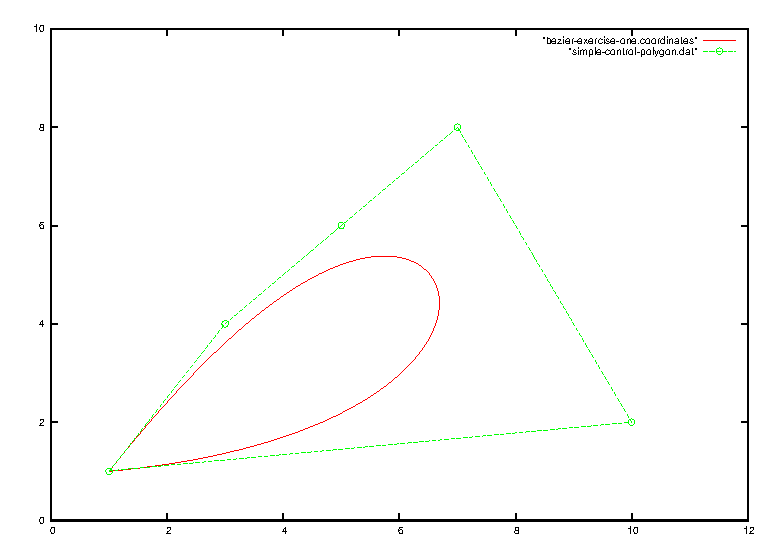
\includegraphics{bezier-deCasteljau-curves/exercise-one}
  \caption{Curve from simple set of control points}
  \label{fig:first-closed-curve}
\end{figure}

\subsection{Curve from parametric specification}
As required in Exercise 3, in \autoref{fig:curve-from-parametric-spec}
we report a Bezier curve matching the following parametric
specification:
\begin{displaymath}
  \left [  \begin{array}{c}
      x(u) \\
      y(u)
    \end{array} \right ] = \left [
    \begin{array}{c}
      1 + u + u^2 \\
      u^3
    \end{array} \right ]
\end{displaymath}
with $u\in[0,1]$. In order to find the control polygon we do simple
reductions with \emph{Maxima}:

\noindent
%%%%%%%%%%%%%%%
%%% INPUT:
\begin{verbatim}
a:v0*(1-t)^3 + v1*3*t*(1-t)^2 + v2*3*(t^2)*(1-t) + v3*t^3;
\end{verbatim}}
%%% OUTPUT:
\definecolor{labelcolor}{RGB}{100,0,0}
\begin{math}\displaystyle
\parbox{8ex}{\color{labelcolor}(\%o1) }
{t}^{3}\,v3+3\,\left( 1−t\right) \,{t}^{2}\,v2+3\,{\left( 1−t\right) }^{2}\,t\,v1+{\left( 1−t\right) }^{3}\,v0
\end{math}


\noindent
%%%%%%%%%%%%%%%
% %%% INPUT:
% \begin{minipage}[t]{8ex}{\color{red}\bf
% \begin{verbatim}
% (%i2)
% \end{verbatim}}
% \end{minipage}
% \begin{minipage}[t]{\textwidth}{\color{blue}
\begin{verbatim}
b:ratsimp(a,t);
\end{verbatim}}
%%% OUTPUT:
\definecolor{labelcolor}{RGB}{100,0,0}
\begin{math}\displaystyle
\parbox{8ex}{\color{labelcolor}(\%o2) }
{t}^{3}\,\left( v3−3\,v2+3\,v1−v0\right) +{t}^{2}\,\left( 3\,v2−6\,v1+3\,v0\right) +t\,\left( 3\,v1−3\,v0\right) +v0
\end{math}

\noindent
%%% INPUT:
\begin{verbatim}
b = 1 + t + t^2 + 0*t^3;
\end{verbatim}}
%%% OUTPUT:
\definecolor{labelcolor}{RGB}{100,0,0}
\begin{math}\displaystyle
\parbox{8ex}{\color{labelcolor}(\%o3) }
{t}^{3}\,\left( v3−3\,v2+3\,v1−v0\right) +{t}^{2}\,\left( 3\,v2−6\,v1+3\,v0\right) +t\,\left( 3\,v1−3\,v0\right) +v0={t}^{2}+t+1
\end{math}


\noindent
%%% INPUT:
\begin{verbatim}
solve([coeff(b, t,3) = 0, coeff(b, t,2) = 1, coeff(b, t,1) = 1,
        coeff(b, t,0) = 1], [v0,v1,v2,v3]);
\end{verbatim}}
%%% OUTPUT:
\definecolor{labelcolor}{RGB}{100,0,0}
\begin{math}\displaystyle
\parbox{8ex}{\color{labelcolor}(\%o4) }
[[v0=1,v1=\frac{4}{3},v2=2,v3=3]]
\end{math}
%%%%%%%%%%%%%%%


\noindent
%%%%%%%%%%%%%%%
%%% INPUT:
\begin{verbatim}
a:y0*(1-t)^3 + y1*3*t*(1-t)^2 + y2*3*(t^2)*(1-t) + y3*t^3;
\end{verbatim}}
%%% OUTPUT:
\definecolor{labelcolor}{RGB}{100,0,0}
\begin{math}\displaystyle
\parbox{8ex}{\color{labelcolor}(\%o5) }
{t}^{3}\,y3+3\,\left( 1−t\right) \,{t}^{2}\,y2+3\,{\left( 1−t\right) }^{2}\,t\,y1+{\left( 1−t\right) }^{3}\,y0
\end{math}
%%%%%%%%%%%%%%%


\noindent
%%%%%%%%%%%%%%%
%%% INPUT:
\begin{verbatim}
b:ratsimp(a,t);
\end{verbatim}}
%%% OUTPUT:
\definecolor{labelcolor}{RGB}{100,0,0}
\begin{math}\displaystyle
\parbox{8ex}{\color{labelcolor}(\%o6) }
{t}^{3}\,\left( y3−3\,y2+3\,y1−y0\right) +{t}^{2}\,\left( 3\,y2−6\,y1+3\,y0\right) +t\,\left( 3\,y1−3\,y0\right) +y0
\end{math}
%%%%%%%%%%%%%%%


\noindent
%%%%%%%%%%%%%%%
%%% INPUT:
\begin{verbatim}
b = t^3;
\end{verbatim}}
%%% OUTPUT:
\definecolor{labelcolor}{RGB}{100,0,0}
\begin{math}\displaystyle
\parbox{8ex}{\color{labelcolor}(\%o7) }
{t}^{3}\,\left( y3−3\,y2+3\,y1−y0\right) +{t}^{2}\,\left( 3\,y2−6\,y1+3\,y0\right) +t\,\left( 3\,y1−3\,y0\right) +y0={t}^{3}
\end{math}
%%%%%%%%%%%%%%%


\noindent
%%%%%%%%%%%%%%%
%%% INPUT:
\begin{verbatim}
solve([coeff(b, t,3) = 1, coeff(b, t,2) = 0, coeff(b, t,1) = 0,
        coeff(b, t,0) = 0], [y0,y1,y2,y3]);
\end{verbatim}}
%%% OUTPUT:
\definecolor{labelcolor}{RGB}{100,0,0}

\begin{math}\displaystyle
\parbox{8ex}{\color{labelcolor}(\%o8) }
[[y0=0,y1=0,y2=0,y3=1]]
\end{math}
%%%%%%%%%%%%%%%

Hence four control points are $\{(1,0), (\frac{3}{4},0), (2,0),
(3,1)\}$.
\begin{figure}
  \centering
  \includegraphics{bezier-deCasteljau-curves/exercise-two}
  \caption{Curve from parametric specification}
  \label{fig:curve-from-parametric-spec}
\end{figure}

\subsection{Splitted curve on a given parameter $u$}
As required in Exercise 4, in \autoref{fig:splitted-curve} we report
the control polygon for the original curve in red, and two sets of
control points with the same cardinality that, used together, build a
Bezier that is the same as the original one. Those sets of points are
obtained via subdivision algorithm (which is a clever implementation of
classic \emph{de Casteljau algorithm}) fixing parameter $\hat{t} =
\frac{1}{4}$: they are colored in green (the relative Bezier in magenta)
and in blue (the relative Bezier in cyan), respectively.
\begin{figure}[h!]
  \centering
  \includegraphics{bezier-deCasteljau-curves/exercise-four}
  \caption{Splitted curve}
  \label{fig:splitted-curve}
\end{figure}

\subsection{Repeating the same control point more times}
As required in Exercise 5, in
\autoref{fig:repeating-same-control-point} we report two Bezier curves: the
red one relative to control points $\{(2,4), (6,12), (10,1),
(12,12)\}$ the green one relative to control points $\{(2,4), (6,12),
(10,1), (10,1), (10,1), (10,1), (12,12)\}$, ie. with the point
$(10,1)$ repeated three more times. We see that curve relative to
the augmented control polygon goes down toward $(10,1)$ more than the
other curve: this can be explained from a probabilistic point of
view, since a Bezier curve can be thought as a \emph{mean} of the control
polygon, hence repeating point $(10,1)$ increases its weight.

\begin{figure}[h!]
  \centering
  \includegraphics{bezier-deCasteljau-curves/exercise-five}
  \caption{Repeating the control point $(10,1)$ three more times}
  \label{fig:repeating-same-control-point}
\end{figure}

\subsection{Increasing degree}
As required in Exercise 6, we start from an original set of control
points, plotted in \autoref{fig:increasing-degree-original-curve}, and
we proceed by increasing degrees of successive Bezier curves three times.
We obtains three augmented set of control points, plotted in
\autoref{fig:some-increased-degrees}, respectively. It is possible to
check the slow convergence for the sequence of polygons to the Bezier
curve and, in \autoref{fig:increasing-degree-does-change-curve}, the
Bezier curves relative to each augmented polygons doesn't change in
shape, ie their set of points equal the original one (we simply plot
those Bezier curves in the same plot and each one is over the others).

\begin{figure}[h!]
  \centering
  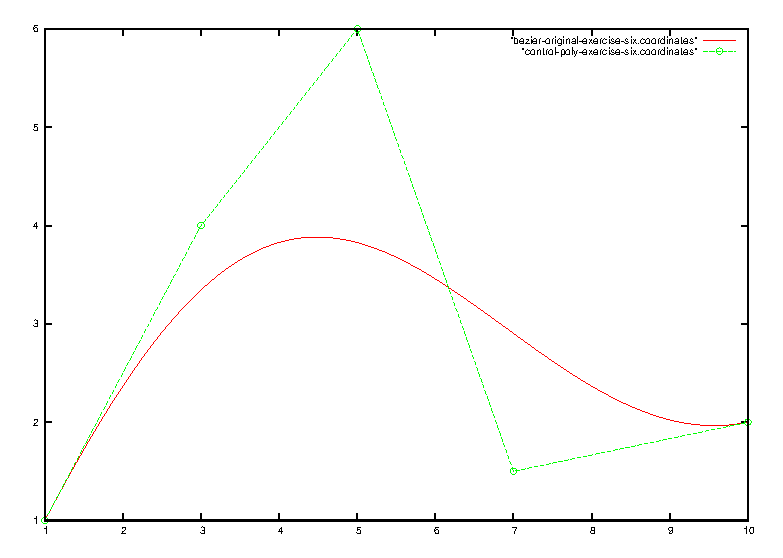
\includegraphics{bezier-deCasteljau-curves/exercise-six-original}
  \caption{Original curve before increasing degree}
  \label{fig:increasing-degree-original-curve}
\end{figure}

\begin{figure}[h!]
  \centering
  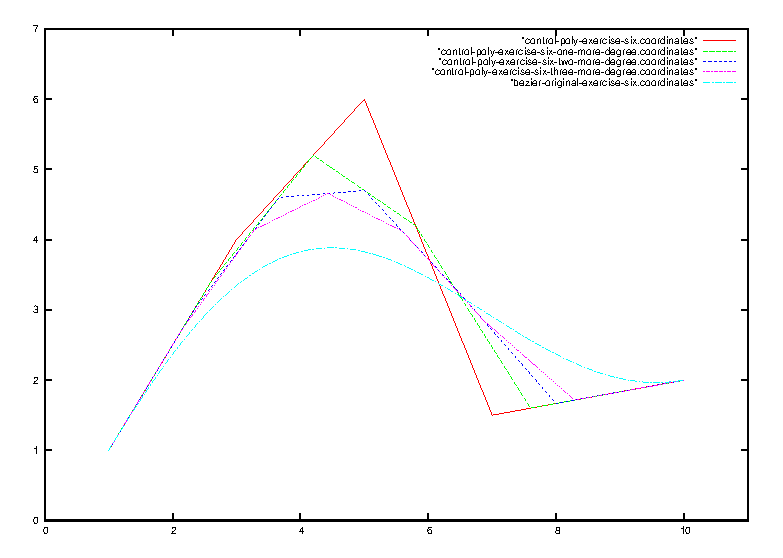
\includegraphics{bezier-deCasteljau-curves/exercise-six-higher-degree-control-poly}
  \caption{Some control polygons, each one with one more degree}
  \label{fig:some-increased-degrees}
\end{figure}

\begin{figure}[h!]
  \centering
  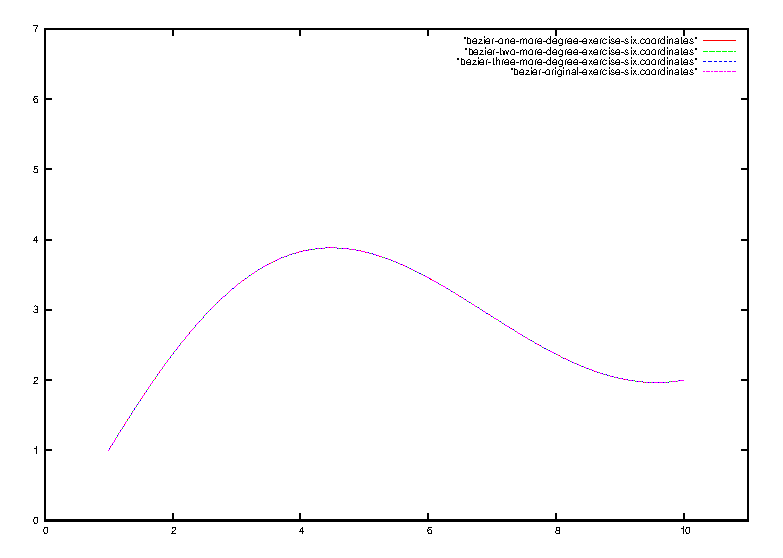
\includegraphics{bezier-deCasteljau-curves/exercise-six-one-more-degree-comparison}
  \caption{Increasing degree doesn't change the Bezier shape}
  \label{fig:increasing-degree-does-change-curve}
\end{figure}

\subsection{Joining curve requiring $\mathcal{C}^0, \mathcal{C}^1, \mathcal{C}^2$}

In this section we report plots about Bezier spline curves,
extending a fixed control net, requiring $\mathcal{C}^0,
\mathcal{C}^1, \mathcal{C}^2$ for each extension, both on the right
(see
\autoref{fig:bezier-spline-right-extension-continuity},
\autoref{fig:bezier-spline-right-extension-tangent},
\autoref{fig:bezier-spline-right-extension-obsculating},
respectively) both on the left (see
\autoref{fig:bezier-spline-left-extension-continuity},
\autoref{fig:bezier-spline-left-extension-tangent},
\autoref{fig:bezier-spline-left-extension-obsculating},
respectively).

\begin{figure}[h!]
  \centering
  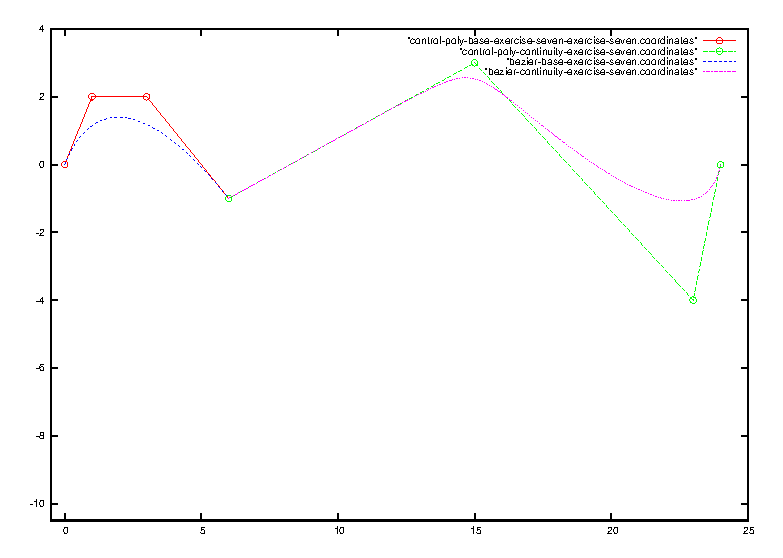
\includegraphics{bezier-deCasteljau-curves/exercise-seven-continuity}
  \caption{Bezier spline curve, requiring $\mathcal{C}^0$, extending on the right}
  \label{fig:bezier-spline-right-extension-continuity}
\end{figure}

\begin{figure}[h!]
  \centering
  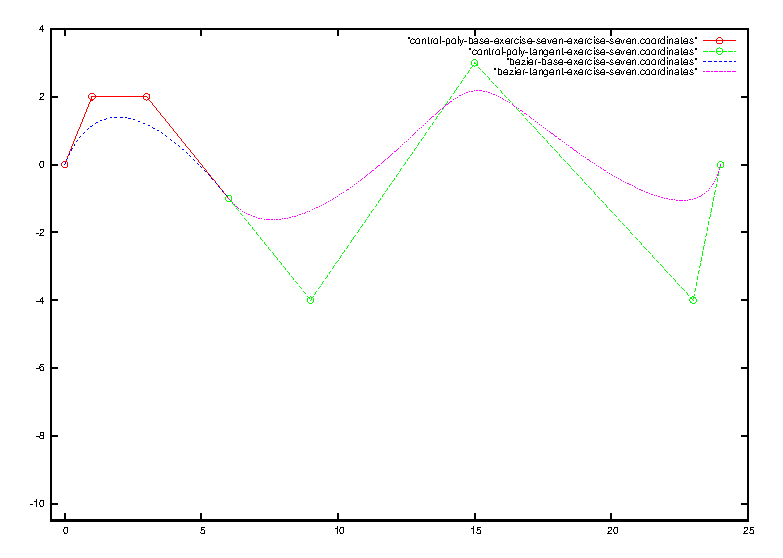
\includegraphics{bezier-deCasteljau-curves/exercise-seven-tangent}
  \caption{Bezier spline curve, requiring $\mathcal{C}^1$, extending on the right}
  \label{fig:bezier-spline-right-extension-tangent}
\end{figure}

\begin{figure}[h!]
  \centering
  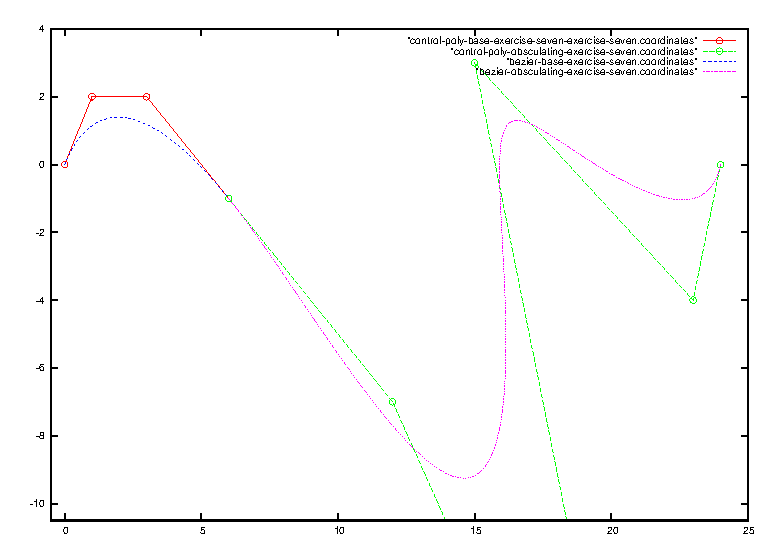
\includegraphics{bezier-deCasteljau-curves/exercise-seven-obsculating}
  \caption{Bezier spline curve, requiring $\mathcal{C}^2$, extending on the right}
  \label{fig:bezier-spline-right-extension-obsculating}
\end{figure}

% 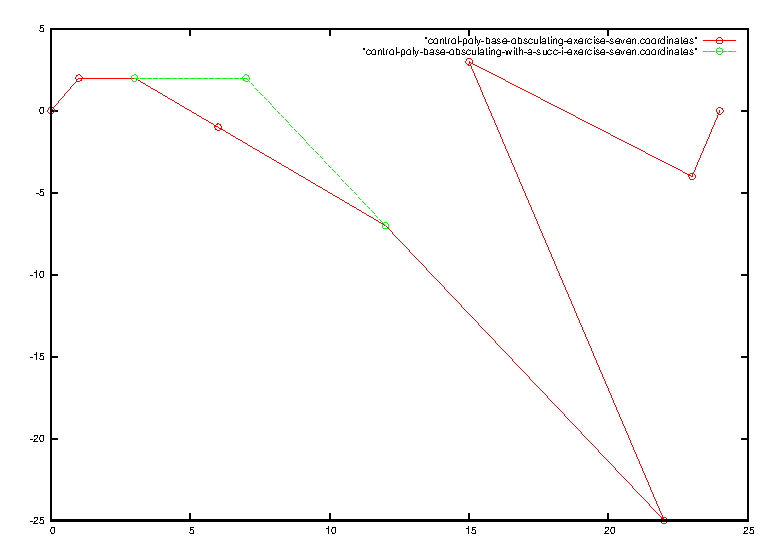
\includegraphics{bezier-deCasteljau-curves/exercise-seven-a_succ_i}

\begin{figure}[h!]
  \centering
  \includegraphics{bezier-deCasteljau-curves/exercise-seven-continuity-left}
  \caption{Bezier spline curve, requiring $\mathcal{C}^0$, extending on the left}
  \label{fig:bezier-spline-left-extension-continuity}
\end{figure}

\begin{figure}[h!]
  \centering
  \includegraphics{bezier-deCasteljau-curves/exercise-seven-tangent-left}
  \caption{Bezier spline curve, requiring $\mathcal{C}^1$, extending on the left}
  \label{fig:bezier-spline-left-extension-tangent}
\end{figure}

\begin{figure}[h!]
  \centering
  \includegraphics{bezier-deCasteljau-curves/exercise-seven-obsculating-left}
  \caption{Bezier spline curve, requiring $\mathcal{C}^2$, extending on the left}
  \label{fig:bezier-spline-left-extension-obsculating}
\end{figure}

% \includegraphics{bezier-deCasteljau-curves/exercise-seven-a_i-left}

\newpage

\subsection{First Polar of a Bezier curve}

In this section we elaborate an extra exercise relative to first derivative
of a Bezier curve and the first step of de Casteljau algorithm.

Let $\mathbf{p}_{1}(t)$ a Bezier curve built over a control net with $n$ points
$\mathbf{b}_{0}^{(1)},\ldots,\mathbf{b}_{n-1}^{(1)}$, respect a fixed parameter $\hat{t}$
after one step of de Casteljau algorithm. Just use the formal definition:
\begin{displaymath}
    \begin{split}
        \mathbf{p}_{1,\hat{t}}(t)  &= \sum_{i=0}^{n-1}{\mathbf{b}_{i}^{(1)}(\hat{t})B_{i}^{n-1}(t)} \\
            &=  \sum_{i=0}^{n-1}{\left( (1-\hat{t})\mathbf{b}_{i}^{(0)} +
                \hat{t}\mathbf{b}_{i+1}^{(0)}\right)B_{i}^{n-1}(t)} \\
            &=  \sum_{i=0}^{n-1}{\left( (1-\hat{t})\mathbf{b}_{i}^{(0)} +
                \hat{t}\mathbf{b}_{i+1}^{(0)} -\left( (1-t)\mathbf{b}_{i}^{(0)} +
                t\mathbf{b}_{i+1}^{(0)}\right)\right)B_{i}^{n-1}(t)} +
                \sum_{i=0}^{n-1}{\mathbf{b}_{i}^{(1)}(t)B_{i}^{n-1}(t)} \\
            &=  \sum_{i=0}^{n-1}{\left( (t-\hat{t})\mathbf{b}_{i}^{(0)} +
                (\hat{t}-t)\mathbf{b}_{i+1}^{(0)}\right)B_{i}^{n-1}(t)} +
                \sum_{i=0}^{n-1}{\mathbf{b}_{i}^{(1)}(t)B_{i}^{n-1}(t)} \\
            &=  (\hat{t}-t)\sum_{i=0}^{n-1}{\left(
                \mathbf{b}_{i+1}^{(0)} - \mathbf{b}_{i}^{(0)}\right)B_{i}^{n-1}(t)} +
                \sum_{i=0}^{n-1}{\mathbf{b}_{i}^{(1)}(t)B_{i}^{n-1}(t)} \\
    \end{split}
\end{displaymath}
where, with little abuse of notation, $\mathbf{b}_{i}^{(1)}(t) =
\left( (1-t)\mathbf{b}_{i}^{(0)} + t\mathbf{b}_{i+1}^{(0)}\right)$.
Recall that $n\sum_{i=0}^{n-1}{\left(
\mathbf{b}_{i+1}^{(0)} - \mathbf{b}_{i}^{(0)}\right)B_{i}^{n-1}(t)}$ is the
first derivative of a Bezier curve, hence:
\begin{displaymath}
    \begin{split}
        \mathbf{p}_{1, \hat{t}}(t)  &= \mathbf{b}_{1, t}(t) +
        \frac{\hat{t}-t}{n}\frac{\partial \mathbf{b}_{0, \hat{t}}(t) }{\partial t}
    \end{split}
\end{displaymath}
So, this is called the ``first polar form'' of Bezier curve $\mathbf{b}_{0, \hat{t}}(t)$
respect parameter $\hat{t}$. Geometrically, the term $\mathbf{b}_{1, t}(t)$ is an affine
combination of points $\mathbf{b}_{0}^{(0)},\ldots,\mathbf{b}_{n}^{(0)}$ respect parameter
$t$ (not $\hat{t}$), hence it is a point also; the term
        $\frac{\hat{t}-t}{n}\frac{\partial \mathbf{b}_{0, \hat{t}}(t) }{\partial t} $
is a vector, so $\mathbf{p}_{1, \hat{t}}(t)$ is a vector applied to a point, yielding a point
as required. It is quite interesting how the polar form combine a point produced using $t$
as parameter with the derivative vector produced using  parameter $\hat{t}$. This derivation
comes from \cite{Farin}, page 73, and we report the output of our implementation in
\autoref{fig:exercise-polar-form}.

\begin{figure}[h!]
  \centering
  \includegraphics{bezier-deCasteljau-curves/exercise-polar}
  \caption{First Polar form of a Bezier curve}
  \label{fig:exercise-polar-form}
\end{figure}

%%%%%%%%%%%%%%%%%%%%%%%%%%%%%%%%%%%%%%%%%%%%%%%%%%%%%%%%%%%%%%%%%%%%%%%%

\newpage

\section{B-Splines curves}

\subsection{Mushrooms from clumped, uniformed and closed partitions}

In this section we report three simple BSpline curves, using
three different knots partitions: \emph{clumped, uniform} and
\emph{cyclic} (see \autoref{fig:clumpled-mushroom},
    \autoref{fig:uniformed-mushroom} and \autoref{fig:closed-mushroom}
respectively). The control polygon doesn't change
  and aims to produce a mushroom in cartoon style, each knot
has multiplicity $1$ (so maximum continuity is required in each junction)
and no control point is repeated.

\begin{figure}[h!]
  \centering
  \includegraphics{b-splines/exercise-zero-clumped.eps}
  \caption{Mushroom from clumped knots partition}
  \label{fig:clumpled-mushroom}
\end{figure}

\begin{figure}[h!]
  \centering
  \includegraphics{b-splines/exercise-zero-uniformed.eps}
  \caption{Mushroom from uniformed knots partition}
  \label{fig:uniformed-mushroom}
\end{figure}

\begin{figure}[h!]
  \centering
  \includegraphics{b-splines/exercise-zero-closed.eps}
  \caption{Mushroom from cyclic knots partition}
  \label{fig:closed-mushroom}
\end{figure}

\subsection{Increasing order $k$ while decreasing \emph{continuity} vector }
As Exercise 1 requires, in \autoref{fig:bspline-exercise-one-clumped} we
report five BSpline curves, each one of them drawn against the same control
net. We modify for each curve its knots partition, formally for curves
$\mathbf{c}_{1},\mathbf{c}_{2},\mathbf{c}_{3},\mathbf{c}_{4}$ and $\mathbf{c}_{5}$
the following extended partitions are used:
\begin{displaymath}
    \begin{split}
        \Delta_{1} &= \lbrace 0,0, \frac{1}{5}, \frac{2}{5},
            \frac{3}{5},\frac{4}{5},1,1 \rbrace \\
        \Delta_{2} &= \lbrace 0,0,0, \frac{1}{4},
            \frac{1}{2},\frac{3}{4},1,1,1 \rbrace \\
        \Delta_{3} &= \lbrace 0,0,0,0,
            \frac{1}{3},\frac{2}{3},1,1,1,1 \rbrace \\
        \Delta_{4} &= \lbrace 0,0,0,0,0,\frac{1}{2},
            1,1,1,1,1 \rbrace \\
        \Delta_{5} &= \lbrace 0,0,0,0,0,0,1,1,1,1,1,1 \rbrace \\
    \end{split}
\end{displaymath}
respectively, and each curve $\mathbf{c}_{i}$ has \emph{degree} $i$. As
we can see, each knots partition is clumped, so the first and last control points
are interpolated and the sequence of curves uses partitions with knots $0$ and $1$
repeated one more time in successive partitions. For lower degree curves, such as
$\mathbf{c}_{1}$, they are quite next to control net, in particular $\mathbf{c}_{1}$
is the control net itself, while curve $\mathbf{c}_{2}$ is tangent to control net
in two segments since it has \emph{order} $3$ and for $t \in [\frac{1}{4}, \frac{1}{2}) =
[t_4, t_5)$ curve $\mathbf{c}_{2}$ has support $[t_2,t_3,t_4]$ where knot $0$
has multiplicity $2$, hence $\frac{\partial \mathbf{c}_{2}(t)}{\partial t}$
lies on direction given by $\mathbf{V}_{3} - \mathbf{V}_{2}$.
The same reasoning can be done for knot $1$.
Finally, the very last partition allow to draw a \emph{Bezier} curve (the yellow one).

\begin{figure}[h!]
  \centering
  \includegraphics{b-splines/exercise-one-clumped.eps}
  \caption{Decreasing the \emph{continuity} vector collapsing in a Bezier }
  \label{fig:bspline-exercise-one-clumped}
\end{figure}

\subsection{Knots' multiplicities against the same control polygon}
In \autoref{fig:bspline-exercise-two} we report plots required by Exercise 2.
This composite picture contains 5 curves according the following specifications,
from top to bottom:
\begin{center}
    \begin{tabular}{ c c }
        order & knots partition \\
        \hline
        4 & $\lbrace 0^{4},1,2,3,4,5,6,7,8,9,10 \rbrace$  \\
        4 & $\lbrace 0^{4},1^{2},2^{2},3^{2},4^{4} \rbrace$  \\
        6 & $\lbrace 0^{6},1,2,3,4,5^{6} \rbrace$  \\
        6 & $\lbrace 0^{6},1,2,3^{2},4^{6} \rbrace$  \\
        8 & $\lbrace 0^{8},1,2,3^{8} \rbrace$  \\
    \end{tabular}
\end{center}
The curve relative to the first row interpolate the first control point
since $0$ has multiplicity $4$ which is the curve's order, while the last
control point isn't interpolated since knots partition ends uniformly.

The curve relative to the second row both interpolate the first control
point due to the multiplicity $k$ of $0$ and is tangent to control net
on the direction $\mathbf{V}_{4} - \mathbf{V}_{3}$ since for $t \in [t_{5}, t_{6}]$
the support is $[t_{2},t_{3},t_{4},t_{5}]$, where $0$ has multiplicity $3 = order -1$.

Curves relative to third and forth rows both interpolate first and last control
points because of clumped partition, while the last one reduce to only two
knots $1,2$, toward Bezier representation.

\begin{figure}[h!]
  \centering
  \includegraphics{b-splines/exercise-two.eps}
  \caption{Knots's multiplicities increased against the same control polygon }
  \label{fig:bspline-exercise-two}
\end{figure}

\subsection{Linearity near doubled control point with a clumped partition}
In \autoref{fig:bspline-exercise-three} we plot curve required for Exercise 3:
a quadratic curve ($order = 3$) with a doubled control point $\mathbf{V}_{3} =
\mathbf{V}_{4} = (1,1)$ over an extended partition
$\Delta = \lbrace 0,0,0, \frac{1}{4},\frac{1}{2},\frac{3}{4},
1,1,1 \rbrace$, a clumped one with no repeated knots.

Lets consider the subcurve $\mathbf{c}_{5}(t)$ for $t \in [t_{5}, t_{6}]$:
\begin{displaymath}
    \mathbf{c}_{5}(t) = \sum_{i=3}^{5}{\mathbf{V}_{i}N_{i,3}(t)}
\end{displaymath}
Since $\mathbf{V}_{4} = \mathbf{V}_{3}$, for $t \in [t_{5}, t_{6}]$,
$\mathbf{c}_{5}(t)$ must lie on the convex hull $\mathbf{V}_{3}, \mathbf{V}_{4},
\mathbf{V}_{5}$ and,  for $t \in [t_{4}, t_{5}]$, $\mathbf{c}_{5}(t)$ must lie
on the convex hull $\mathbf{V}_{2}, \mathbf{V}_{3}, \mathbf{V}_{4}$, it does follow
that $\mathbf{c}_{5}(t_{5})$ has to lie in their intersection, therefore vertex
$\mathbf{V}_{4}$, interpolating it.

Moreover, $\mathbf{c}_{5}(t)$ has two linear segment between
$\mathbf{V}_{2}, \mathbf{V}_{3}$ and $\mathbf{V}_{4}, \mathbf{V}_{5}$,
both of them join in $t_{4}, t_{6}$ with continuity $\mathcal{C}^{1}$.


\begin{figure}[h!]
  \centering
  \includegraphics{b-splines/exercise-three.eps}
  \caption{Linearity toward $(1,1)$ due to ``linearized'' convex hull}
  \label{fig:bspline-exercise-three}
\end{figure}

\subsection{Two clumped partitions, different \emph{continuity} vectors
    and same control polygon}
In \autoref{fig:bspline-exercise-four} we report two curves required by Exercise 4.
Both of them have $order = 4$ and a control net with a doubled point
$\mathbf{V}_{3} = \mathbf{V}_{4}$, while the former (colored green)
is over a knots partition
$\Delta_{1} = \lbrace 0,0,0,0,\frac{1}{4}, \frac{3}{4}, 1,1,1,1 \rbrace$
(having simple knots, no repeated one), the latter (colored blue) is over
a knots partition
$\Delta_{2} = \lbrace 0,0,0,0,\frac{1}{2}, \frac{1}{2}, 1,1,1,1 \rbrace$ (having
knot $\frac{1}{2}$ doubled). Let define the following subcurves of the former:
\begin{displaymath}
    \begin{split}
        \mathbf{c}_{4}(t) &= \sum_{i=1}^{4}{\mathbf{V}_{i}N_{i,4}(t)}, \quad
            t \in [t_{4}, t_{5}] \\
        \mathbf{c}_{5}(t) &= \sum_{i=2}^{5}{\mathbf{V}_{i}N_{i,4}(t)}, \quad
            t \in [t_{5}, t_{6}] \\
        \mathbf{c}_{6}(t) &= \sum_{i=3}^{6}{\mathbf{V}_{i}N_{i,4}(t)}, \quad
            t \in [t_{6}, t_{7}] \\
    \end{split}
\end{displaymath}
Now $\mathbf{c}_{5}^{\prime}(t_{5}) = \mathbf{c}_{4}^{\prime}(t_{5})$, so the
curve interpolate a point on the segment with extrema $\mathbf{V}_{2}, \mathbf{V}_{3}$
and it is tangent to the control net in $t_{5}$. On the other hand,
$\mathbf{c}_{6}^{\prime}(t_{6}) = \mathbf{c}_{5}^{\prime}(t_{6})$, so the
curve interpolate a point on the segment with extrema $\mathbf{V}_{4}, \mathbf{V}_{5}$
and it is tangent to the control net in $t_{6}$.
Finally, observe that the curve doesn't
interpolate the doubled control point $\mathbf{V}_{3} = \mathbf{V}_{4}$.

The previous argument doesn't apply to the second curve because its
knots partition is not simple, it contains a double knot.

\begin{figure}[h!]
  \centering
  \includegraphics{b-splines/exercise-four.eps}
  \caption{Same control polygon with doubled $(0,6)$ againts two clumped partitions}
  \label{fig:bspline-exercise-four}
\end{figure}

\subsection{Increasing clumped partitions for increasing occurrences of a control point}
In Exercise 5 it is required to provide three extended knots partitions in
order to draw cubic curves reported in \autoref{fig:bspline-exercise-five}.
Each curve is defined against the ``same'' control net, having the middle vertex
of the top row repeated one, two, three times respectively. Our choice of knots
partitions, each clumped since interpolation of first and last control points
is requested:
\begin{displaymath}
    \begin{split}
        \Delta_{1} &= \lbrace 0,0,0,0,\frac{1}{2},1,1,1,1 \rbrace \\
        \Delta_{2} &= \lbrace 0,0,0,0,\frac{1}{3},\frac{2}{3},1,1,1,1 \rbrace \\
        \Delta_{3} &= \lbrace 0,0,0,0,\frac{1}{4},\frac{1}{2},\frac{3}{4},1,1,1,1 \rbrace \\
    \end{split}
\end{displaymath}


\begin{figure}[h!]
  \centering
  \includegraphics{b-splines/exercise-five.eps}
  \caption{Three B-Splines, each for $1,2,3$ occurrences of $(0,1)$ respectively }
  \label{fig:bspline-exercise-five}
\end{figure}

\subsection{Two B-Splines from two closed partitions}
In this last section we report two closed curves having $order = 4$ over
two cyclic knots partitions, in \autoref{fig:bspline-exercise-six-first}
and \autoref{fig:bspline-exercise-six-second}, respectively.

\begin{figure}[h!]
  \centering
  \includegraphics{b-splines/exercise-six-first-closed.eps}
  \caption{A first B-Spline from a closed partition }
  \label{fig:bspline-exercise-six-first}
\end{figure}

\begin{figure}[h!]
  \centering
  \includegraphics{b-splines/exercise-six-second-closed.eps}
  \caption{A second B-Spline from a closed partition }
  \label{fig:bspline-exercise-six-second}
\end{figure}

\newpage

\begin{thebibliography}{}

\bibitem{Julia} Open Source Project,
  \emph{Julia language}, \url{http://julialang.org/}

\bibitem{Farin} Gerald Farin,
  \textit{Curves and surfaces for CAGD, Fifth Edition}


\end{thebibliography}



\end{document}
